\documentclass[reqno]{article}

% if you need to pass options to natbib, use, e.g.:
%     \PassOptionsToPackage{numbers, compress}{natbib}
% before loading neurips_2020

% ready for submission
% \usepackage{styles}

% to compile a preprint version, e.g., for submission to arXiv, add add the
% [preprint] option:
\usepackage[final, nonatbib]{styles}

% to compile a camera-ready version, add the [final] option, e.g.:
%     \usepackage[final]{neurips_2020}

% to avoid loading the natbib package, add option nonatbib:
% \usepackage[nonatbib]{styles}

\usepackage[utf8]{inputenc} % allow utf-8 input
\usepackage[T1]{fontenc}    % use 8-bit T1 fonts
\usepackage{hyperref}       % hyperlinks
\usepackage{url}            % simple URL typesetting
\usepackage{booktabs}       % professional-quality tables
\usepackage{amsfonts}       % blackboard math symbols
\usepackage{bbm}
\usepackage{nicefrac}       % compact symbols for 1/2, etc.
\usepackage{microtype}      % microtypography
\usepackage{graphicx}
\usepackage{tabularx}
\usepackage{booktabs}
\usepackage{multirow}
\usepackage{array}
\graphicspath{ {./images/} }

\usepackage[numbers]{natbib}
\bibliographystyle{apalike}

\newcolumntype{C}[1]{>{\centering\arraybackslash}m{#1}}
\newcolumntype{A}{>{\centering\arraybackslas}p{0.25\textwidth}}
\newcommand{\ra}[1]{\renewcommand{\arraystretch}{#1}}

\title{Image Classification with Deep Learning}

\author{
	Timoshenko Dmitrii\\
	Department of Statistics\\
	University of California, Berkeley\\
	\texttt{timoshenko\_dmitrii@berkeley.edu} \\
}

\begin{document}
	
	\maketitle
	
	\begin{abstract}
				This project explores various Deep Learning approaches for image classification in sports. The dataset includes 100 classes of different sports, with a limited number of examples for training, validation, and testing. We experiment with different CNN architectures, including state-of-the-art models, to evaluate their performance on the test set. Additionally, we investigate techniques to improve model accuracy, such as data augmentation, increasing the depth of classifier layers, and blending with boosting. Through our experiments, we aim to identify the best-performing methods for sports image classification\footnote{Code can be found here: https://github.com/ronega/STAT254-project}.
	\end{abstract}
	
	\section{Introduction}
	Image classification is an important task in computer vision, with numerous applications in fields such as robotics, surveillance, and medical imaging. In recent years, deep learning techniques have been at the forefront of image classification, achieving state-of-the-art results in a variety of domains. Sports imagery is a particularly interesting domain for image classification, as it poses unique challenges due to the high variability of the images and the need to distinguish between similar poses and actions. While there have been several studies on sports image classification, this paper aims to explore different methods for this task. Specifically, the performance of various deep learning architectures and preprocessing techniques will be investigated on a dataset of images from different sports. The goal is to provide insights into which methods are most effective for sports image classification and to contribute to the development of more accurate and robust classification systems for sports imagery
	
	\section{Data}
	
	The key aspect of this project was collecting a suitable dataset to train the models. The dataset of 100 different sports was obtained from Kaggle\footnote{\url{https://www.kaggle.com/datasets/gpiosenka/sports-classification}}, which consists of 100 training samples, 5 validation samples, and 5 test samples for each class. The images in the dataset are colorful and non-centered, with the color scheme being RGB. Each image comprises three channels of red, green, and blue colors, which are combined to create the final image. However, the non-centered nature of the data suggests that the images may not be perfectly aligned and may require some preprocessing before they can be used in machine-learning models. Moreover, unlike datasets like MNIST, where the images are well-centered, some traditional computer vision methods may not show good results in sports image classification tasks. Therefore, I used deep learning approaches, which I discuss in detail later in the paper. 
	
	To provide a better understanding of the dataset, Figure \ref{examples} shows some examples of the images.
	
		\begin{figure}[h]
			\centering
			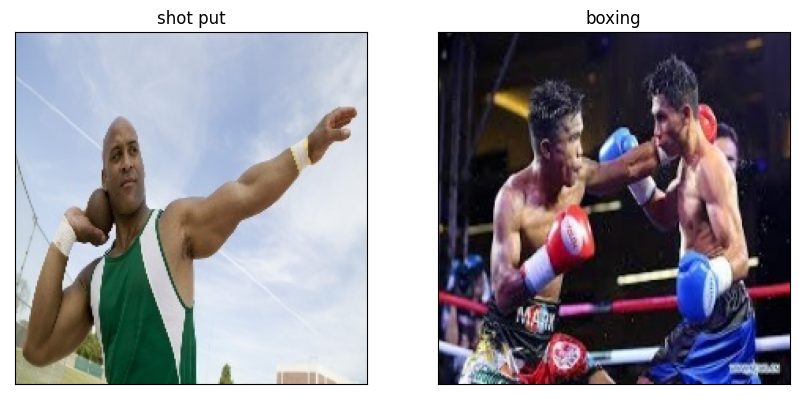
\includegraphics[width=0.5\linewidth]{Example_of_images.png}
			\caption{Examples of images in the dataset}
			\label{examples}
		\end{figure}
	
	\section{Methods}
	
	In this section, I describe the methods I used to achieve the best performance. There are some reasons, why traditional machine learning methods can't be used:
	
	\begin{itemize}
		\item The data is non-centered, making it difficult for traditional methods such as tree-based and regression models to create appropriate boundaries to classify the images effectively
		\item The images in the dataset have a high resolution of 224x224x3, making it computationally expensive to use traditional models even after grayscaling. 
		\item Color is a critical feature in sports image classification. For instance, the color difference between soccer and basketball images is significant and plays a crucial role in improving the prediction power of the models.
	\end{itemize}
	
	Given the challenges posed by the sports image classification task, I decided to use deep learning methods, and specifically, a Convolutional Neural Network (CNN), as it is one of the most suitable models for this task.
	
	\subsection{Pretrained CNN: ConvNet as fixed feature extractor}
	
	\textbf{Motivation.} Since the dataset is relatively small, building a neural network from scratch would not be an ideal approach. Deep learning methods typically require a large amount of data to achieve good performance.\footnote{However, I trained my own model. Accuracy was too low: 0.296, which is higher than I get from ShuffleNet}. Therefore, I decided to use pre-trained CNN models instead. The main idea behind this approach is to use a pre-trained CNN model with frozen main layers (known as CNN codes), and only train the classifier layer with randomly initialized weights.
	
	\textbf{Training.} I used various CNN architectures as fixed feature extractors and modified only the number of neurons in the last layer to correspond with the total number of classes in the dataset (i.e., 100). Each model was trained on a dataset consisting of 100 samples for each class and validated on 5 images for each class after every epoch to evaluate the model's performance and prevent overfitting. Prior to training, the images were normalized to enhance model performance.
	
	Main parameters of the training procedure described in Table \ref{training-params}. For calculation a loss after each epoch, I used cross entropy (Eq. \ref{cross_ent}), with averaging it over number of samples in batch.
	
	\begin{equation}
		\label{cross_ent}
		Loss_n = -w_{y_n}log\frac{exp(x_{n,y_n})}{\sum_{c=1}^C exp(x_{n,c})}
	\end{equation}

\begin{table}[ht]
	\caption{Training parameters for CNN models}
	\label{training-params}
	\centering
	\renewcommand{\arraystretch}{1.1}
		\begin{tabular}{
				>{\centering\arraybackslash}p{3.5cm}
				c
				p{6cm}}
			\toprule
				\textbf{Parameter}     & \textbf{Value}     & \textbf{Comment}    \\ \midrule
				Batch size & 32  & Number of images to proceed in one forward step    \\
			No. of epoches     & 100 &  Total number of epoches. All models were fully trained before the number \\
			Early stop     &   5     & If no improvement on validation dataset for this number of epochs, training will be stopped  \\
			Loss function & Cross entropy & Most common criteria in classification \\
			Optimization algorithm & SGD/Adam & Optimizer used in the model. For some models SGD worked better than Adam \\
			Learning rate & 0.001 &  Regulates the speed of the weight adjustment\\
			Weights & ImageNet & All weights for pre-trained models were frozen. Last layer had random weight initialization \\
			\bottomrule
		\end{tabular}
\end{table}

I chose different models, including the most recent one, to check their performance on my dataset. The training was completed on an NVIDIA A100 GPU, and the training time in Table \ref{results-native} is measured in minutes. The accuracy metric for the test is defined as the share of correctly predicted images in the test dataset (Eq. \ref{accuracy}).

I chose several pretrained models to test their performance. Before discussing the results, I will briefly explain their architectures.

\begin{equation}
	\label{accuracy}
	Accuracy = \frac{\sum_{i=1}^n \mathbbm{1}(\hat{y}_i \neq y_i)}{n}
\end{equation}

\subsubsection{AlexNet}

	AlexNet is a deep convolutional neural network developed by Alex Krizhevsky, Ilya Sutskever, and Geoffrey Hinton \citep{NIPS2012_c399862d}. It consists of 8 layers, including 5 convolutional layers and 3 fully connected layers. The input to the network is an image of size 224x224x3, where 3 represents the RGB channels. This model serves as a good baseline, as it learns quickly and provides an expected accuracy threshold.

\subsubsection{ResNet}

	ResNet (short for "Residual Network") is a deep convolutional neural network architecture that was introduced by Kaiming He, Xiangyu Zhang, Shaoqing Ren, and Jian Sun in 2015 \citep{he2015deep}. It was designed to address the problem of vanishing gradients in very deep neural networks by introducing skip connections that allow information to bypass certain layers in the network. In many applications, this model shows great results with relatively low computational costs.

\subsubsection{Inception}

	The Inception architecture, also known as GoogleNet, is a convolutional neural network architecture that was introduced by researchers at Google in 2014 \citep{szegedy2015rethinking}. The authors proposed some key differences from previous networks:
	
	\begin{itemize}
		\item Increase the model not only in depth, but also in width
		\item Reduce the number of layers with a transition from a large number of parameters to a smaller number, i.e. avoid bottlenecks
		\item Small convolutions can be effective as nearby pixels are often highly correlated, so reducing the image size can be done without significant losses in accuracy
	\end{itemize}

The architecture differs greatly from AlexNet and ResNet, so I decided to test its performance on my dataset.


\subsubsection{SuffleNet}

ShuffleNet is a convolutional neural network architecture that was introduced by researchers at Megvii (also known as Face++) in 2017 \citep{ma2018shufflenet}. ShuffleNet uses a channel shuffle technique to reduce the number of parameters and the computational cost of the network while balancing accuracy with computational efficiency.

\subsubsection{EfficientNet} 

EfficientNet is a convolutional neural network architecture that was introduced by researchers at Google in 2020 \cite{tan2020efficientnet, tan2021efficientnetv2}. The EfficientNet architecture achieves this goal by using a compound scaling approach, where the network is scaled up or down in terms of depth, width, and resolution based on a set of scaling coefficients. The model demonstrated good performance in similar problems.

\subsubsection{Vision Transformer (ViT) }

The Vision Transformer (ViT) is a deep learning architecture introduced by Google in 2020 \citep{dosovitskiy2021image}. It is based on the Transformer architecture that was originally proposed for natural language processing tasks, but has been adapted for use in computer vision tasks. The ViT architecture works by transforming an input image into a sequence of tokens that are then processed by a series of Transformer blocks. Novel architecture that I also wanted to test on my dataset.

\begin{table}
	\caption{Training Results}
	\label{results-native}
	\centering
	\renewcommand{\arraystretch}{1.1}
	\begin{tabular}{lcc}
		\toprule
		&\multicolumn{2}{c}{Metrics}                   \\
		\cmidrule(r){2-3}
		Model     & Accuracy on test     & Training Time\\
		\midrule
		AlexNet (2012)    & 0.86       & \textbf{8} \\
		ResNet50 (2015)    & \textbf{0.97}       & 23  \\
		ResNet152 (2015)      & 0.94      & 38   \\
		Inception V3 (2015)      & 0.92       & 47  \\
		SuffleNet V2 (2018)     & \textbf{0.03} & 21 \\
		EfficientNet B3 (2019)  & 0.88     & 17  \\
		EfficientNet B6 (2019)  & 0.80     & 24  \\
		EfficientNetV2-S (2021)   &  0.87   & 36 \\
		EfficientNetV2-L (2021)   &  0.94   & 34 \\		
		ViT-B (2021)   &  0.95   & 24 \\
		ViT-L (2021)   &  0.92   & 89 \\		
		\bottomrule
	\end{tabular}
\end{table}

\textbf{Results.} Table \ref{results-native} summarizes the training procedure and shows that the ResNet50 architecture performed the best among all models tested. Despite parameter tuning attempts using different optimizers, learning rates, and schedulers, the ShuffleNet V2 model did not improve its predictive power. Furthermore, larger versions of some models (ResNet, EfficientNet, ViT) did not outperform their smaller counterparts as expected. One possible reason for this is that larger models are better suited for recognizing more complex patterns in images, which may not be necessary for this particular dataset.

Also, Figure \ref{wrong-images} demonstrates the wrongly labeled images. Overall, the results seem very good--even for humans, it is possible to make a mistake on these images.

	\begin{figure}[ht]
	\centering
	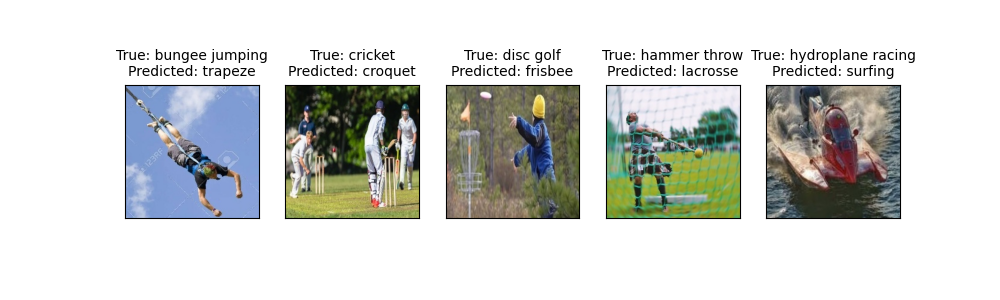
\includegraphics[width=1\linewidth]{Wrong_images}
	\caption{Examples of wrong predictions}
	\label{wrong-images}
\end{figure}


\subsection{Pretrained CNN: Data Augmentation}

\textbf{Motivation.} Since the initial dataset is small, increasing the number of samples with augmentation is a reasonable way to improve the predictive power of CNN models.

\textbf{Training.} Two versions of augmentation were implemented: one using two filters, each with a probability of 0.5, and the other using several filters with different probabilities. \footnote{Augmentation was used only on the training dataset.} The description of filters can be found in Table \ref{aug_filters}, and Figure \ref{augmentation_example} shows the filters used in training. Some filters were used with a probability less than 0.5 because they could change the picture too much for the models, so they were included with low probability to prevent overfitting. Filters that could change colors too much were not used because color is one of the most important features of the dataset, as mentioned in the motivation for using pretrained CNN models.

\textbf{Results.} The most important outcomes of the method are as follows:

\begin{itemize}
	\item The training time increased for most models, as expected, because transforming images requires more time to process them before actual training.
	\item For some models (Inception V3, EfficientNetV2-S/L, AlexNet), the quality of predictions decreased. Again, the reason for this is the small size of the initial dataset.
	\item Unexpectedly, the training time for some models with several filters increased compared to two filters. This was likely because I wasn't the only user of the GPU and couldn't control its usage.
	\item Overall, in most cases, using two filters for the given dataset is a better option, as models are less likely to miss details and don't require much time to train. The latter could be improved with the use of other technical solutions, such as Albumentations (example: \url{https://albumentations.ai}).
\end{itemize}

		\begin{figure}[ht]
			\centering
			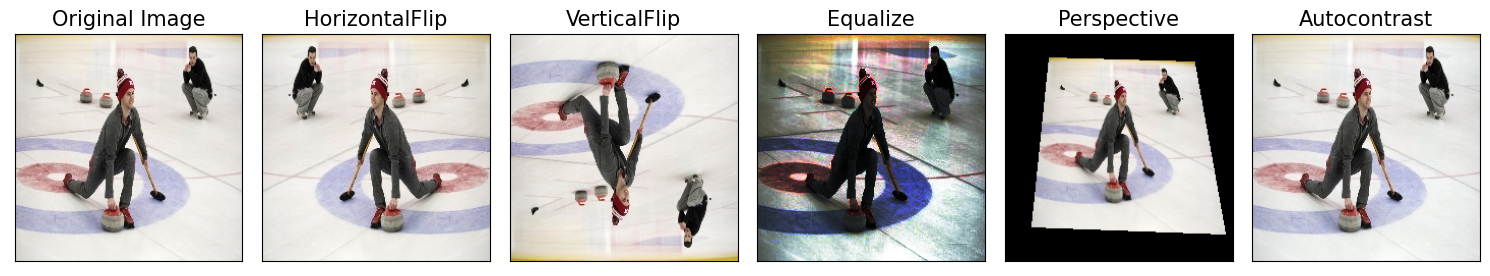
\includegraphics[width=1\linewidth]{Augmentation.png}
			\caption{Examples of augmentation}
			\label{augmentation_example}
		\end{figure}

\subsection{ResNet50: Different Classifier}

\textbf{Motivation.} Another method I used to attempt to increase the predictive power was to increase the depth of the classifier, as the feature extraction might be good enough to improve it further.

\textbf{Training.} I used the ResNet50 architecture as a feature extractor since it showed the best accuracy among all models, and its training time is not as long as that of larger models. To make the classifier layer deeper, I included more fully connected and dropout layers with ReLU and ELU as non-linear activation functions. \footnote{Some clarifications on the notation: D - dropout; L - FC layer; Re - ReLU activation function; Elu - ELU activation function}. The loss function and most of the parameters are the same as in previous sections. The changes to the initial architecture are illustrated in Figure \ref{feature_extraction} (visuals created by the author).

\textbf{Results.} Unfortunately, making the classifier deeper did not improve the predictive power as expected. In all cases, accuracy decreased by 1.5-2 percentage points compared to the initial ResNet50 architecture as a feature extractor. I tried different specifications and have described them in Table \ref{results-resnet50-new_classifier}.

	\begin{figure}[ht]
		\centering
		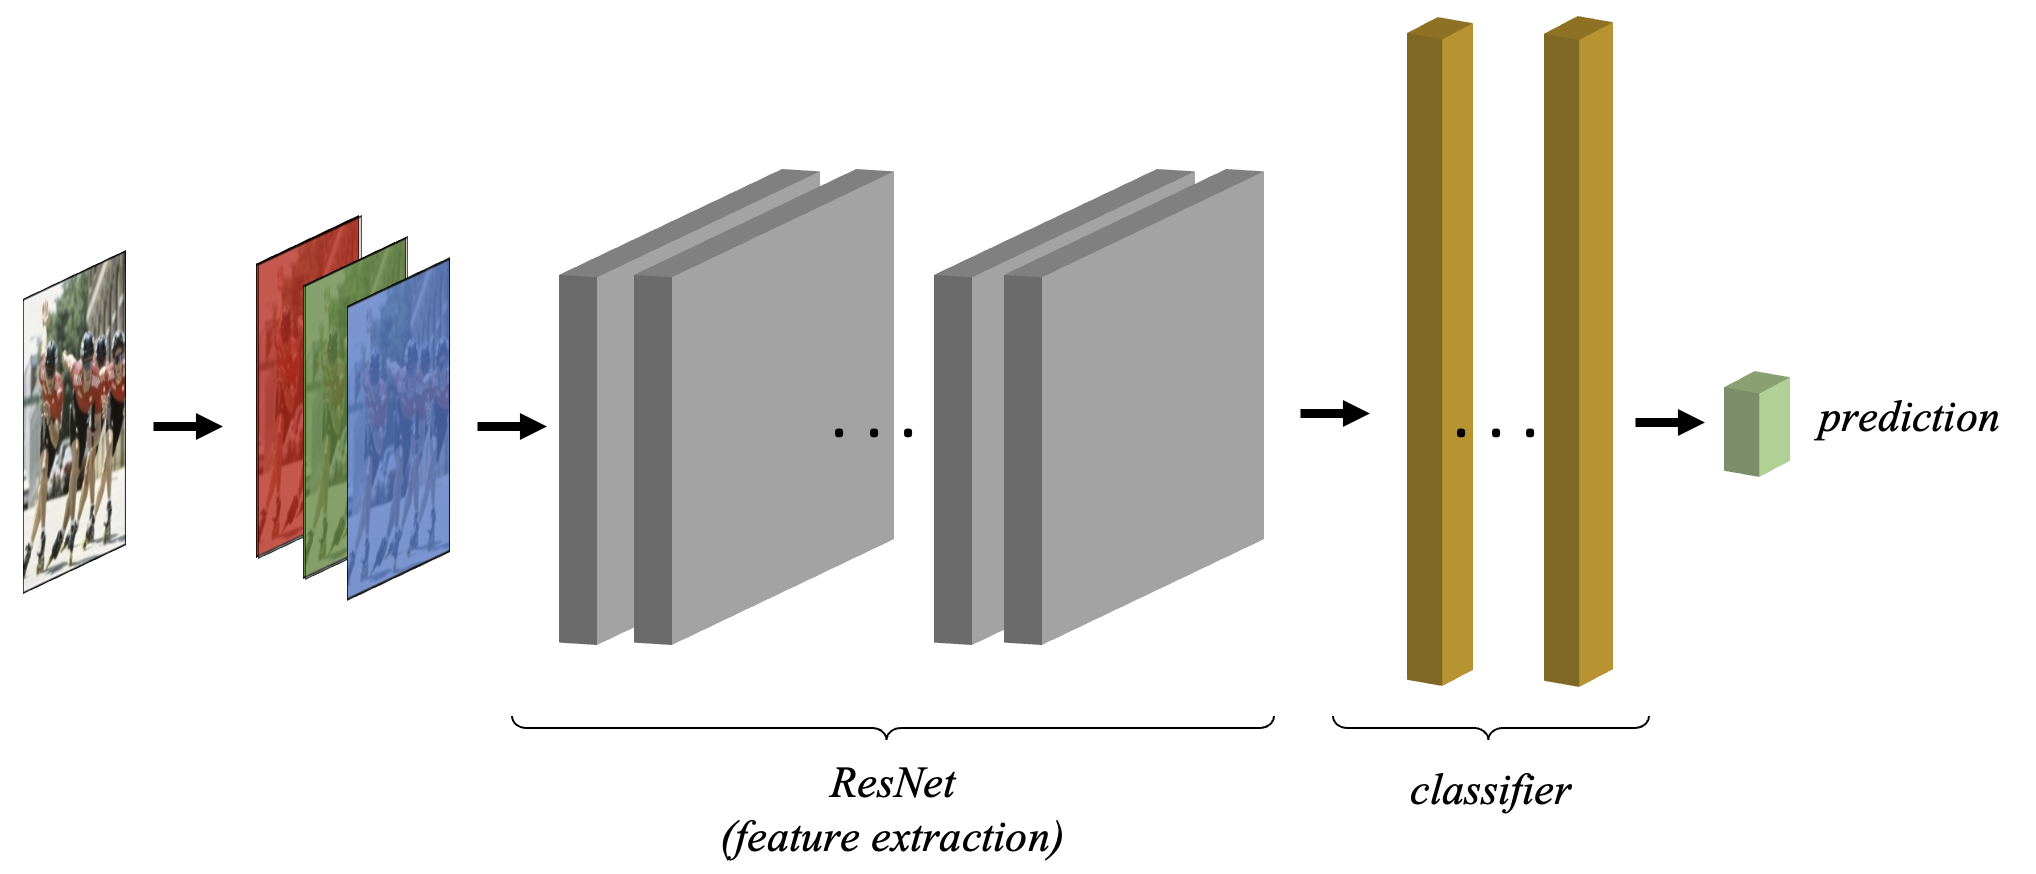
\includegraphics[width=0.7\linewidth]{CNN_feature_exct}
		\caption{ResNet50 as a feature extractor, combined with newly trained classifier}
		\label{feature_extraction}
	\end{figure}

\subsection{Blending: CNN with Boosting}

\textbf{Motivation.} Another method I attempted to improve the classification power of the models was to combine their predictions to build one strong classifier. I used trained models as a feature extractor and built another model that identifies the most important features and uses them to make a final decision on the class label. Figure \ref{boosting} demonstrates this idea.

\textbf{Training.} The training procedure is as follows:
\begin{enumerate}
	\item Train five different neural networks.
	\item Instead of predicting the class, obtain the outputs before the softmax layer. This yields 100 features from each model for each image, resulting in 500 features for each picture.
	\item Without losing the train/valid/test split, train a boosting model to increase the overall accuracy of the models.
	\item Predict the class of the test images and evaluate the new accuracy.
\end{enumerate}

I tried different specifications and I describe them in Table \ref{results-catboost}.

	\begin{figure}[ht]
	\centering
	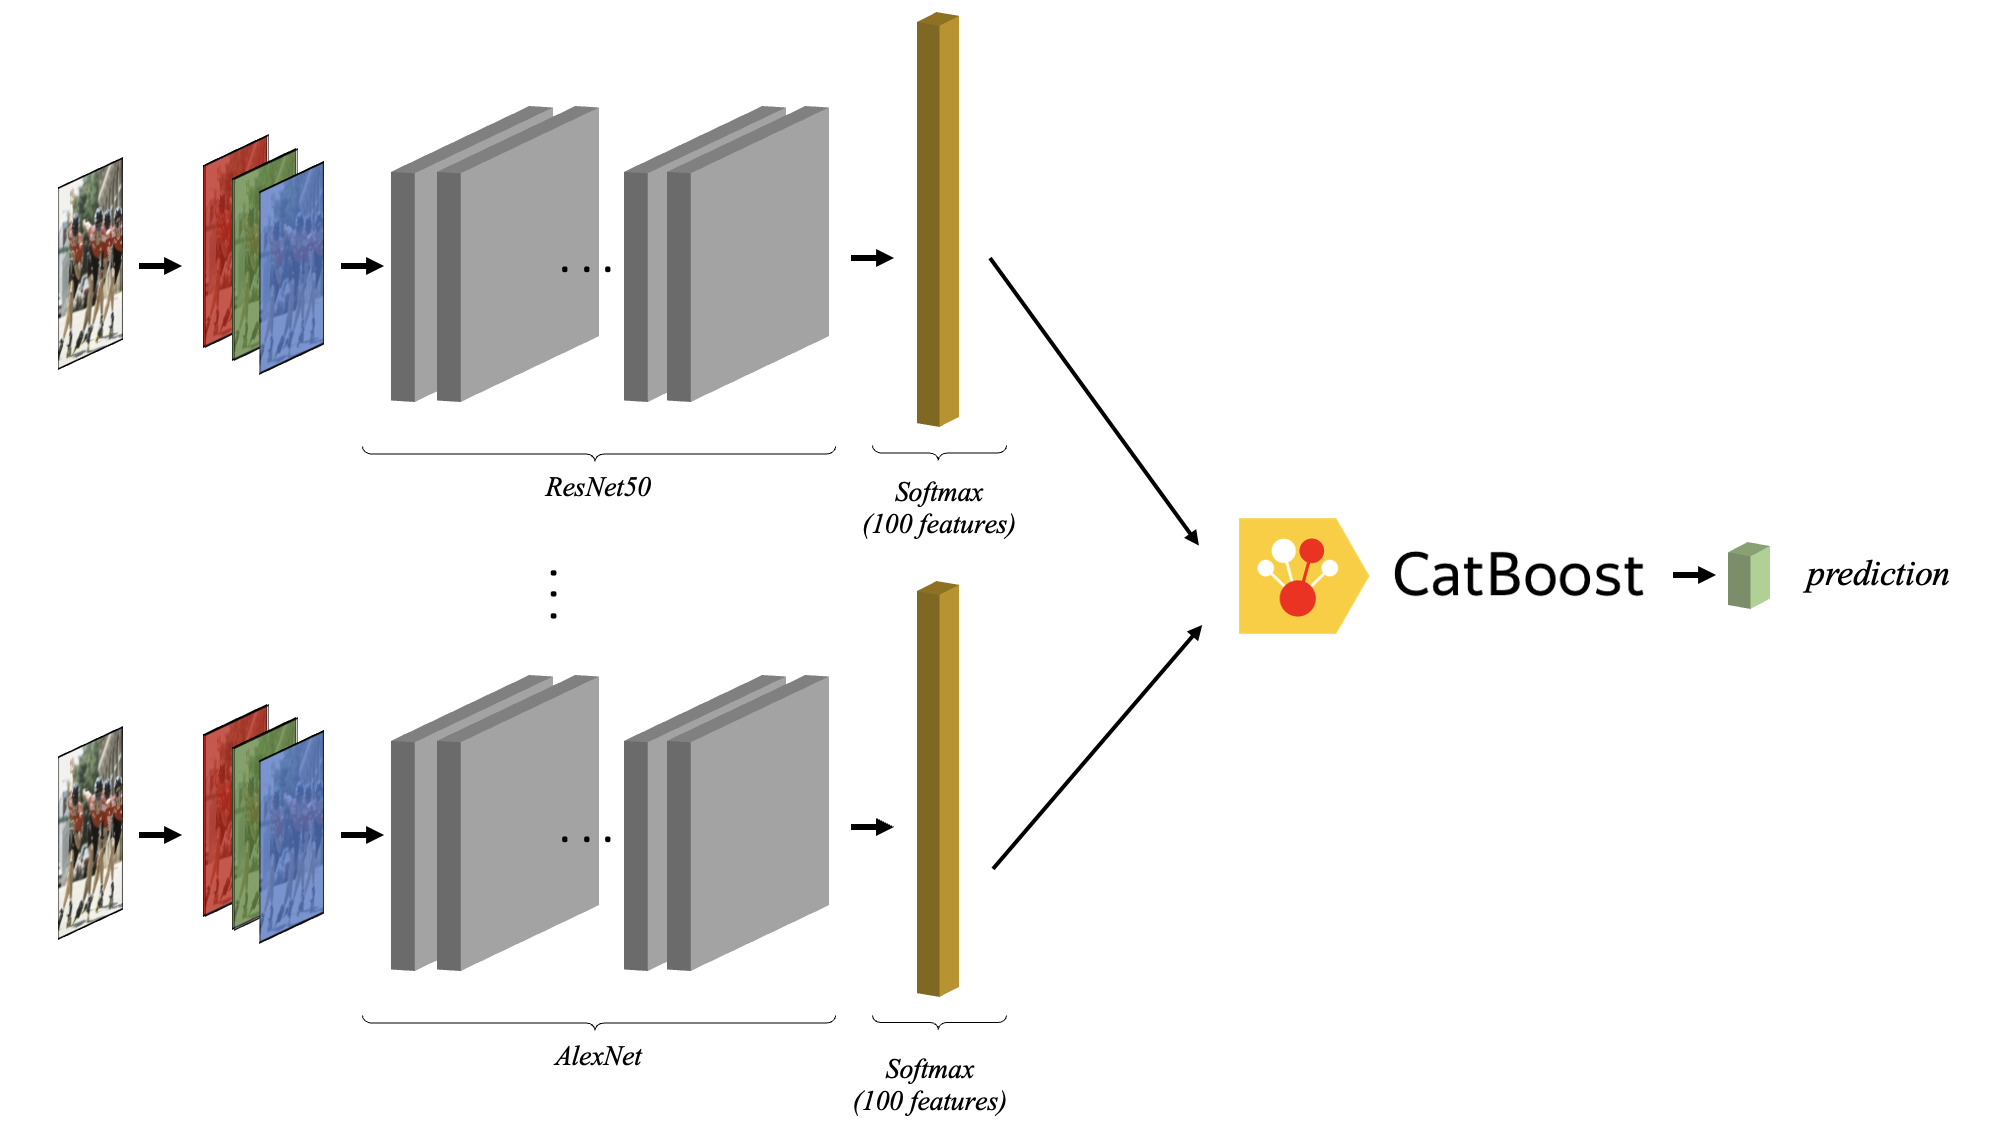
\includegraphics[width=0.8\linewidth]{Catboost}
	\caption{Several CNN models combined to make a prediction after boosting}
	\label{boosting}
\end{figure}

\textbf{Results.} This method didn't increase overall accuracy of models, even given the fact that in data there was an output from ResNet50 architecture, which showed 0.97 accuracy. Interesting, that after checking confusion matrix, I noticed the model predict \texttt{air\_hockey}  too often: among 51 errors for different images, the model wrongly predicted \texttt{air\_hockey}, instead of correct class. Possible solution here: drop this class, but even after removing the class, nothing changes -- accuracy is still relatively low, 0.84.

\section{Conclusion}

In this project, I tried different models for image classification and found that the ResNet50 architecture performed very well on my data, achieving high performance (0.97) in a relatively short training time. Various techniques that are usually employed to improve model accuracy didn't yield significant improvements, possibly due to the small size of the dataset and the already high accuracy of the ResNet50 model. Areas for potential future research could include:

\begin{itemize}
	\item Parameter tuning for models.
	\item Unfreeze layers and train them as well (now it is impossible due to high computational costs). A good thing to try would be different learning rates for layers -- higher for the classifier and lower for the feature extractor.
	\item Increase the dataset with other images using web parsing.
\end{itemize}

\newpage

\bibliography{reference.bib}
	
	\newpage
	\section*{Appendix}
	\appendix
	
	\setcounter{table}{0}
	\renewcommand{\thetable}{A\arabic{table}}
	\begin{table}[ht]
		\caption{Filters for augmentation}
		\label{aug_filters}
		\centering
		\renewcommand{\arraystretch}{1.1}
		\begin{tabular}{
				>{\centering\arraybackslash}p{2.5cm}
				>{\centering\arraybackslash}p{2.5cm}
				>{\centering\arraybackslash}p{2.2cm}
				>{\centering\arraybackslash}p{2.2cm}
				>{\centering\arraybackslash}p{2.2cm}}
			\toprule
			\textbf{Filter}     & \textbf{Probability}     & \textbf{Comment}  & \textbf{Setting 1} & \textbf{Setting 2}\\ \midrule
			RandomHorizontalFlip & 0.5  & Flip an image horizontally    & Yes  & Yes\\
			RandomVerticalFlip & 0.5 &  Flip an image vertically & Yes  & Yes\\
			RandomEqualize & 0.1 &  Equalizes the histogram of image & No  & Yes\\
			RandomPerspective & 0.3 &Performs perspective transform & No  & Yes\\
			RandomAutocontrast & 0.3& Applies autocontrast & No  & Yes\\
			\bottomrule
		\end{tabular}
	\end{table}

\newpage
\begin{center}
\begin{table}
	\caption{Training Results}
	\label{results-native_full}
	\centering
	\renewcommand{\arraystretch}{1.1}
	\begin{tabular}{
			l 
			>{\centering\arraybackslash}p{1.5cm}
			>{\centering\arraybackslash}p{1.3cm}
			>{\centering\arraybackslash}p{1.5cm}
			>{\centering\arraybackslash}p{1.3cm} 
			>{\centering\arraybackslash}p{1.5cm}
			>{\centering\arraybackslash}p{1.3cm}}
		\toprule
			& \multicolumn{2}{c}{Native}& \multicolumn{2}{c}{Two filters} &\multicolumn{2}{c}{Multiple filters} \\
		\cmidrule(lr){2-3}\cmidrule(lr){4-5}\cmidrule(lr){6-7}
		Model  & Training time & Accuracy & Training time  & Accuracy & Training time & Accuracy\\
		\midrule
		AlexNet (2012)           & 9  & 0.87 & 25  & 0.86 & 9   & 0.80 \\
		ResNet50 (2015)           & 23 & 0.97 & 61  & 0.96 & 42  & 0.97 \\
		ResNet152 (2015)          & 38 & 0.94 & 114 & 0.93 & 88  & 0.94 \\
		Inception V3 (2015)      & 47 & 0.92 & 163 & 0.78 & 110 & 0.79 \\
		SuffleNet V2 (2018) & 21 & 0.03 & 112 & 0.03 & 139 & 0.02\\
		EfficientNet B3 (2019)   & 17 & 0.89 & 47  & 0.89 & 37  & 0.90 \\
		EfficientNet B6 (2019)    & 23 & 0.80 & 110 & 0.80 & 109 & 0.79 \\
		EfficientNetV2-S (2021)    & 36 & 0.88 & 84  & 0.84 & 63  & 0.86 \\
		EfficientNetV2-L (2021)   & 33 & 0.94 & 107 & 0.93 & 106 & 0.94 \\
		ViT-B (2021)            & 24 & 0.95 & 98  & 0.93 & 86  & 0.93 \\
		ViT-L (2021)          & 89 & 0.92 & 212 & 0.88 & 160 & 0.89 \\
		\bottomrule
	\end{tabular}
\end{table}
\end{center}


\newpage
\begin{center}
	\begin{table}
		\caption{Training Results}
		\label{results-resnet50-new_classifier}
		\centering
		\renewcommand{\arraystretch}{1.1}
		\begin{tabular}{
				>{\centering\arraybackslash}p{2cm}
				>{\centering\arraybackslash}p{2cm}
				>{\centering\arraybackslash}p{2cm}
				>{\centering\arraybackslash}p{2cm}
				>{\centering\arraybackslash}p{2cm} 
				>{\centering\arraybackslash}p{2cm}}
			\toprule
			Model  & DLReDL & DLReDLReDL & DLReDL  & DLEluDL & DLReDLReDL\\
			\midrule
			Learning Rate & 0.0005& 0.0001& 0.001& 0.0005& 0.0005\\
			Optimizer & Adam & Adam & SGD & Adam \\
			\midrule
			CNN               & ResNet50                               & ResNet50 								   & ResNet50 								  & ResNet50 								& ResNet50  \\
			Layer 1           &  Dropout 								 & Dropout 								   	   & Dropout  									& Dropout 									 & Dropout  \\
			Layer 2          & FC 2048$\rightarrow$1024 & FC 2048$\rightarrow$1024 &  FC 2048$\rightarrow$1024 & FC 2048$\rightarrow$1024 & FC 2048$\rightarrow$1500  \\
			Layer 3          & ReLU 								  	   & ReLU 									      & ReLU 										  & ELU 										  & ReLU  \\
			Layer 4          & Dropout 									 & Dropout 								      & Dropout 									& Dropout 									 & Dropout  \\
			Layer 5          &  FC 1024$\rightarrow$100   & FC 1024$\rightarrow$512     & FC 1024$\rightarrow$100     & FC 1024$\rightarrow$100     & FC 1500$\rightarrow$750  \\
			Layer 6          & \dots 	  									& ReLU     										& \dots 										  &  \dots 										  & ReLU  \\
			Layer 7          & \dots 	  									& Dropout     								   & \dots 											&  \dots 										 & Dropout  \\
			Layer 8          & \dots 	  									& FC 512$\rightarrow$100          & \dots 										   &  \dots 									 & FC 750$\rightarrow$100  \\
			\midrule
			Epochs to train & 19 & 16 & 48 & 11 & 10 \\
			Accuracy     & 95.8 & 95.8 & 96.21 & 96.01 & 96.41\\
			\bottomrule
		\end{tabular}
	\end{table}
\end{center}

\newpage

\begin{center}
	\begin{table}
		\caption[Caption for LOF]{Training results from blending\textsuperscript{}}
		\small\textsuperscript{} After parameter turning. Unrestricted model (when maximum depth isn't defined) didn't show good result
		\label{results-catboost}
		\centering
		\renewcommand{\arraystretch}{1.1}
		\begin{tabular}{
				>{\centering\arraybackslash}p{2.49cm}
				>{\centering\arraybackslash}p{2cm}
				>{\centering\arraybackslash}p{2cm}
				>{\centering\arraybackslash}p{2cm}
				>{\centering\arraybackslash}p{2cm} 
				>{\centering\arraybackslash}p{2cm}}
			\toprule
			  & Model 1 & Model 2 & Model 3   & Model 4 & Model 5 \\
			\midrule
			Loss function & CrossEntropy & CrossEntropy& CrossEntropy& CrossEntropy& CrossEntropy \\
			Learning Rate & 0.8 & 0.8 & 0.8 & 0.8 & 0.8 \\
			Max Depth & 5 & 5 & 2 & 2 & 5 \\
			L2 Regularization & 5 & 10 & 10 & 15 & 15 \\
			\midrule
			Accuracy     & 0.88 & 0.84 & 0.81 & 0.83 & 0.86 \\
			\bottomrule
		\end{tabular}
	\end{table}
\end{center}


\end{document}